\subsection{Transfer to Contract Fields}
\label{sec:eval:cuad}
We construct a source-span field task from CUAD~\citep{ref_cuad}. Its five fields are document name, agreement date, effective date, expiration date or initial term, and governing law. Contracts must contain at most one distinct whitespace-normalized reference value per field and no more than 40,000 source characters. We retain the full source and verify annotation offsets. Twenty official-training contracts form the development set. The fixed eligibility conditions yield 56 official-test contracts; we use all of them. This evaluates shorter, single-value contracts rather than the full CUAD question-answering task.
The four outputs are initial extraction, simple repair, indexed repair, and indexed re-extraction. Both repair arms receive the same initial graph. Indexed arms add deterministic field-anchor windows while retaining the full source. All arms use the same Gemma model, field definitions and 4,000-token completion limit. Before collection, we fix JSON-fence handling and assign document IDs by code. We use one development round without changing prompts or eligibility before testing. This comparison isolates source context and access to an old graph; it does not evaluate the sequential selector.
\begin{table}[t]
\centering
\caption{CUAD contract-field results on 56 test documents. F1 uses whitespace-normalized exact source spans. Lost counts reference-correct initial facts removed from the output. Initial creation cost is separate from each repair call.}
\label{tab:cuad}
\small
\begin{tabular}{lrrrr}
\toprule
Output & F1 (\%) & Lost & New incorrect & Requests \\
\midrule
Initial extraction & 46.76 & 0 & 0 & 59 \\
Simple repair & 43.35 & 7 & 2 & 71 \\
Indexed repair & 44.84 & 5 & 12 & 69 \\
Indexed re-extraction & 44.12 & 8 & 32 & 71 \\
\bottomrule
\end{tabular}
\end{table}
The primary paired indexed-repair minus indexed-extraction difference is 0.72 F1 points (95\% document-bootstrap interval [-4.80, 6.48]; paired sign-flip $p=0.810$). The test produces 224 outputs from 270 actual requests including retries. Failed outputs remain empty graphs in scoring. Exact source-span agreement measures agreement with CUAD annotations; independent semantic review of edits remains pending.
\begin{figure}[t]
\centering
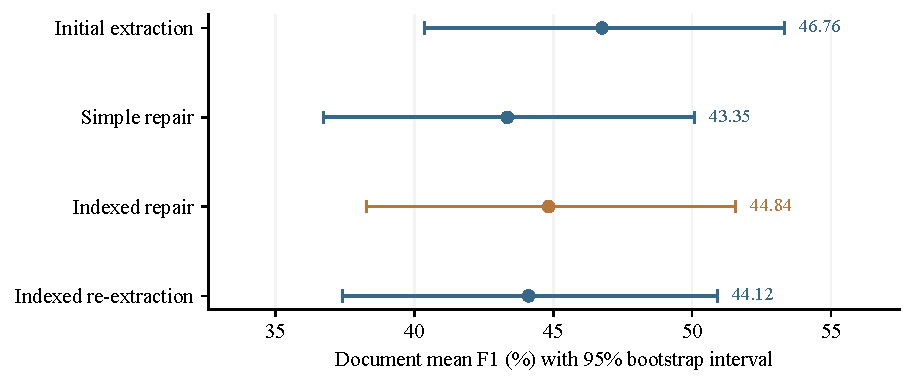
\includegraphics[width=0.88\textwidth]{figure/experiments/cuad_contracts.pdf}
\caption{Contract-field comparison. Points are document mean F1; bars are marginal 95\% document-bootstrap intervals. The primary comparison uses a paired interval reported in the text.}
\label{fig:cuad}
\end{figure}
